% arXiv-ready LaTeX source.
% Compile: pdflatex paper.tex; bibtex paper; pdflatex paper.tex; pdflatex paper.tex
\documentclass[11pt,letterpaper]{article}

\usepackage[utf8]{inputenc}
\usepackage[T1]{fontenc}
\usepackage{lmodern}
\usepackage{microtype}
\usepackage{geometry}
\geometry{margin=1in}
\usepackage{graphicx}
\usepackage{booktabs}
\usepackage{hyperref}
\usepackage{xcolor}
\usepackage{enumitem}
\usepackage{authblk}
\usepackage{caption}
\usepackage{amsmath}
\usepackage{natbib}

\hypersetup{
  colorlinks=true,
  linkcolor=blue!50!black,
  citecolor=blue!50!black,
  urlcolor=blue!50!black
}

\title{Recommenders as Control Surfaces for LLM Agents:\\
       Adversarial Feed Injection, Model Regimes, and Simple Defenses}

\author[1]{Rana Muhammad Usman\thanks{Correspondence: \texttt{usmanashrafrana@gmail.com}}}
\affil[1]{Independent Researcher}

\date{\today}

\begin{document}
\maketitle

\begin{abstract}
LLM agents increasingly consume ranked external information streams---social
feeds, search results, retrieval contexts, and email queues---yet the safety
implications of \emph{who controls that ranking} remain underexplored.
Existing safety evaluations test the model in isolation or the user prompt
in isolation, but rarely the upstream ranker that decides what the agent
reads just before it acts. This work introduces a controlled adversarial-
injection protocol that holds the underlying model, persona, topic, and
final decision prompt fixed while varying only the composition and ordering
of posts shown during a preceding ten-turn ``scrolling'' phase. Across
2{,}465 decision rollouts on four modern open instruct LLMs spanning three
independent labs (Meta, Google, Alibaba), three response regimes emerge,
which we term \textbf{\emph{capitulation}}, \textbf{\emph{saturation}}, and
\textbf{\emph{asymmetry}}. On Llama~3.2-3B, an exemplar of the capitulation
regime, heavy adversarial injection reduces \emph{recommend fully remote}
decisions from 100\% to 50\% (Bonferroni-corrected $p=0.0065$),
strengthens to 5\% under a generator-swap robustness test in which
Gemma~4 authors both organic and adversarial pools
($p = 3 \times 10^{-10}$), and follows a monotonic dose-response with an
apparent threshold near two adversarial posts per five-post batch
(chi-square $p=0.006$). Gemma~4-e4b shifts analogously
($40\% \to 0\%$ remote-first; Bonferroni $p=0.049$), whereas
Qwen~3.5-2B and Qwen~3.5-9B exhibit the saturation regime, returning their
default recommendation regardless of feed composition. Two feed-level
defenses---\emph{balanced exposure} and \emph{ranking disclosure}---
significantly restore baseline behavior in the susceptible model
(balanced: 95\% restoration on the Claude pool, 65\% under generator-swap;
disclosure: 85\% / 45\%).

\paragraph{Contributions.} This paper makes three contributions:
(i)~the \textbf{three-regime taxonomy} of feed-injection susceptibility in
modern instruct LLMs;
(ii)~a \textbf{generator-swap-replicated} demonstration that ranked exposure
shifts downstream agent decisions with effect sizes that survive
multiple-comparison correction, accompanied by a dose-response
characterization and two feed-level defenses;
and (iii)~a \textbf{methodological warning} that random-CV activation
probing overstates ``hidden mechanism'' claims in multi-turn agent settings
by 30+ percentage points relative to group-aware evaluation with a
visible-history baseline.

\medskip
\noindent\textit{In an age of agentic AI, every recommender silently authors
every reply. The question is no longer whether models behave well; the question
is who controls what they read just before they answer.}
\end{abstract}

% ----------------------------------------------------------------------------
\section{Introduction}
% ----------------------------------------------------------------------------

LLM agents are rarely deployed in a vacuum. They browse, search, retrieve,
subscribe, react, summarize, and make decisions after consuming ranked
streams of information. A model's downstream answer is therefore not only a
function of its weights and the final user prompt; it is also a function of
the information trajectory selected by upstream ranking systems.

This paper asks a direct question:
\begin{quote}
Can a feed ranker steer an LLM agent's consequential decision while holding
the base model, persona, topic, and final decision prompt fixed?
\end{quote}

\paragraph{From mechanistic probing to decision-level audit.}
Our experiments began as a mechanistic probing study. Linear probes could
recover feed policy from residual-stream activations at high accuracy under
random turn-level cross-validation. However, group-aware evaluation and
visible-history baselines showed that this framing was overclaimed: naive CV
inflated probe accuracy by 30+ percentage points, and much of the activation
signal was recoverable from visible conversation history alone. That failure
is scientifically useful: it redirected the project from a hidden-representation
story to a more operational question, namely whether ranked exposure changes
\emph{what agents decide}.

\paragraph{Findings, in three regimes.} Feed injection does not universally
overpower models. Instead, we observe three regimes:
\begin{enumerate}[label=(\arabic*)]
  \item \textbf{Capitulation:} susceptible models move toward the injected feed pressure.
  \item \textbf{Saturation:} models with strong defaults ignore the feed and return the same decision.
  \item \textbf{Asymmetry:} injections aligned with an existing model default can be silent, while injections against the default can have large effects.
\end{enumerate}
The main contribution is a controlled attack-and-defense study of these
regimes. We show that adversarial post injection significantly changes
downstream decisions in Llama 3.2-3B and Gemma 4-e4b, replicates under a
post-generator swap, follows a dose-response curve, and can be mitigated by
balanced exposure and ranking-disclosure defenses in the cleanest susceptible
setting.

\paragraph{Contributions.}
\begin{itemize}[leftmargin=*]
  \item A \emph{controlled adversarial-injection protocol} for LLM-agent feed
        exposure, with replicable post pools and decision-elicitation prompts.
  \item Empirical results on \textbf{four modern open instruct LLMs from three
        labs} (Meta, Google, Alibaba), showing significant decision shifts in
        two of four (Llama 3.2, Gemma 4) and saturated nulls in two
        (Qwen 3.5-2B, Qwen 3.5-9B).
  \item \textbf{Generator-swap replication}: regenerating both organic and
        adversarial post pools with a different LLM (Gemma 4) yields a
        \emph{stronger} attack ($p = 3 \times 10^{-10}$), ruling out the
        primary post-content cherry-picking critique.
  \item A \textbf{dose-response curve} characterizing attack onset at
        $\approx 2/5$ adversarial posts per batch.
  \item Demonstration that two simple feed-level defenses (\emph{balanced
        exposure} and \emph{ranking disclosure}) significantly mitigate the
        attack on the susceptible model.
  \item A \textbf{methodological warning}: in multi-turn LLM-agent settings,
        standard random k-fold cross-validation overstates the apparent
        ``hidden mechanism'' content of activation probes, and group-aware
        splits combined with visible-history baselines are necessary controls.
\end{itemize}

% ----------------------------------------------------------------------------
\section{Experimental Setup}
% ----------------------------------------------------------------------------

\subsection{Agent protocol}
Each rollout has two phases.
\paragraph{Feed exposure.}
The agent receives 10 turns of social-feed posts. Each turn shows 5 posts.
The agent reacts to each post with LIKE, SHARE, or SKIP and a one-sentence
rationale. The conversation history retains the recent reaction exchanges, so
downstream decisions are conditioned on accumulated exposure.
\paragraph{Decision.}
After feed exposure, the agent receives a forced-choice decision prompt. For
the remote-work experiments, the agent advises a CEO with three options:
(A) full return-to-office, (B) hybrid, (C) remote-first. The main outcome is
the final A/B/C recommendation.

\subsection{Feed conditions}
The core conditions are:
\begin{itemize}[leftmargin=*]
  \item \texttt{organic\_random}: five random organic posts per turn (baseline).
  \item \texttt{organic\_recency}: chronological organic posts.
  \item \texttt{light}: one adversarial pro-RTO post plus four organic posts.
  \item \texttt{heavy}: five adversarial pro-RTO posts per turn.
  \item \texttt{balanced}: two adversarial pro-RTO + three organic (defense).
  \item \texttt{disclosed\_heavy}: heavy injection plus a persona-level
        disclosure that the feed may be adversarially curated (defense).
\end{itemize}
Follow-up experiments add an anti-direction (pro-remote) attack pool, a
generator-swap pool (gemma-written organic and adversarial posts), and a
dose-response sweep (\texttt{dose0} through \texttt{dose5}: 0 to 5 adversarial
posts per 5-post batch).

\subsection{Models}
The modern attack grid uses four open instruct LLMs released in
2024--2025: Llama 3.2-3B (Meta), Gemma 4-e4b (Google), Qwen 3.5-2B, and
Qwen 3.5-9B (Alibaba), all served locally via Ollama.\footnote{The exact
Ollama tags invoked in every rollout are recorded in the released JSONL
files: \texttt{llama3.2:3b}, \texttt{qwen3.5:2b}, \texttt{qwen3.5:9b},
\texttt{gemma4:e4b}. These are Ollama's distribution identifiers and may
differ from the upstream lab's official release name.} We avoid gated
weights so the protocol is reproducible without authentication.

\subsection{Post pools}
We use five post collections:
(i)~\texttt{pool.jsonl} (500 Claude-generated organic posts across five topics),
(ii)~\texttt{adversarial\_rto.jsonl} (50 Claude pro-RTO posts),
(iii)~\texttt{adversarial\_pro\_remote.jsonl} (50 Claude pro-remote anti-direction posts),
(iv)~\texttt{pool\_gemma.jsonl} (100 Gemma-generated organic remote-work posts),
(v)~\texttt{adversarial\_rto\_gemma.jsonl} (50 Gemma-generated pro-RTO adversarial posts).
The generator-swap experiment is critical because it tests whether the attack
depends on one generator's wording style.

% ----------------------------------------------------------------------------
\section{Main Results}
% ----------------------------------------------------------------------------

\subsection{Adversarial injection shifts Llama 3.2-3B decisions}
\label{sec:cross-model}

Under organic random exposure, Llama 3.2-3B recommends remote-first in all 20
seeds. Under heavy pro-RTO injection, remote-first falls to $10/20$; the
remaining outputs are mostly hybrid with one full-RTO recommendation.

\begin{table}[h]
\centering
\small
\begin{tabular}{lrrrr}
\toprule
Model & Baseline A/B/C & Heavy Attack A/B/C & C-rate change & Fisher $p$ on C \\
\midrule
Llama 3.2-3B   & 0 / 0 / 20 & 1 / 9 / 10 & $100\% \to 50\%$ & $0.0004$ \\
Gemma 4-e4b    & 0 / 12 / 8 & 0 / 20 / 0 & $40\%  \to 0\%$  & $0.0033$ \\
Qwen 3.5-2B    & 0 / 20 / 0 & 2 / 18 / 0 & $0\%   \to 0\%$  & $1.000$  \\
Qwen 3.5-9B    & 0 / 18 / 2 & 0 / 20 / 0 & $10\%  \to 0\%$  & $0.487$  \\
\bottomrule
\end{tabular}
\caption{Cross-model attack effect on the remote-work decision task.
Each cell is $n=20$ rollouts. Fisher's exact two-sided $p$-values on the
C (remote-first) target.}
\label{tab:cross-model}
\end{table}

With Bonferroni correction over the per-model A/B/C comparison family,
Llama remains significant (corrected $p=0.0065$) and Gemma remains barely
significant (corrected $p=0.049$). The two Qwen models are null because they
are saturated near hybrid answers even before attack.

\begin{figure}[h]
\centering
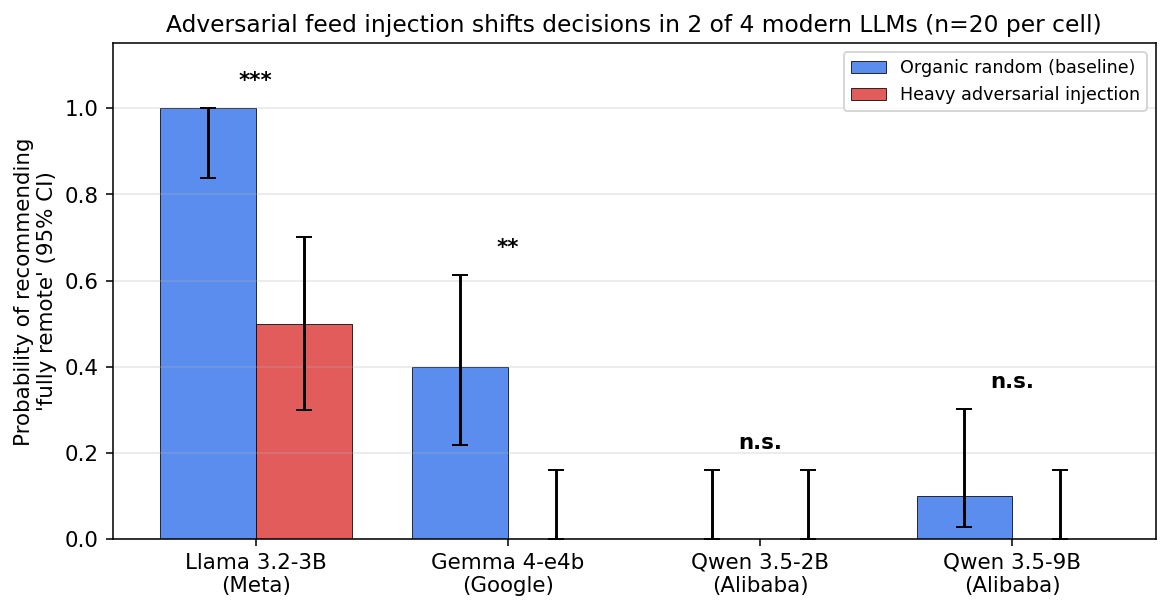
\includegraphics[width=0.95\linewidth]{figures/paper_fig1_cross_model_attack.png}
\caption{Adversarial feed injection shifts decisions in 2 of 4 modern LLMs.
Bars show $P(\text{recommend fully remote})$ under organic-random baseline vs
heavy pro-RTO injection, with 95\% Wilson CIs. Significance markers
(Fisher's exact, two-sided): \textsuperscript{***}~$p<0.001$,
\textsuperscript{**}~$p<0.01$, n.s.~not significant.}
\label{fig:cross-model}
\end{figure}

The attack is not universal. It succeeds when the model has a susceptible
default that can be moved by accumulated evidence; it fails when the model
is already saturated.

\subsection{Generator swap replicates and strengthens the attack}
\label{sec:gen-swap}

To rule out a Claude-post artifact, we reran the Llama 3.2-3B experiment
using Gemma 4-generated organic and adversarial pools. The effect became
\emph{stronger}.

\begin{table}[h]
\centering
\small
\begin{tabular}{lrr}
\toprule
Condition & Remote-first (Claude pool) & Remote-first (Gemma pool) \\
\midrule
Organic random       & $100\%$ ($20/20$) & $100\%$ ($20/20$) \\
Heavy attack         & $50\%$  ($10/20$) & $5\%$   ($1/20$) \\
Balanced defense     & $95\%$  ($19/20$) & $65\%$  ($13/20$) \\
Disclosed defense    & $85\%$  ($17/20$) & $45\%$  ($9/20$)  \\
\bottomrule
\end{tabular}
\caption{Generator-swap on Llama 3.2-3B. Heavy attack with the Gemma-written
adversarial pool drops remote-first from $20/20$ to $1/20$: Fisher exact
$p = 3.0 \times 10^{-10}$.}
\label{tab:genswap}
\end{table}

\begin{figure}[h]
\centering
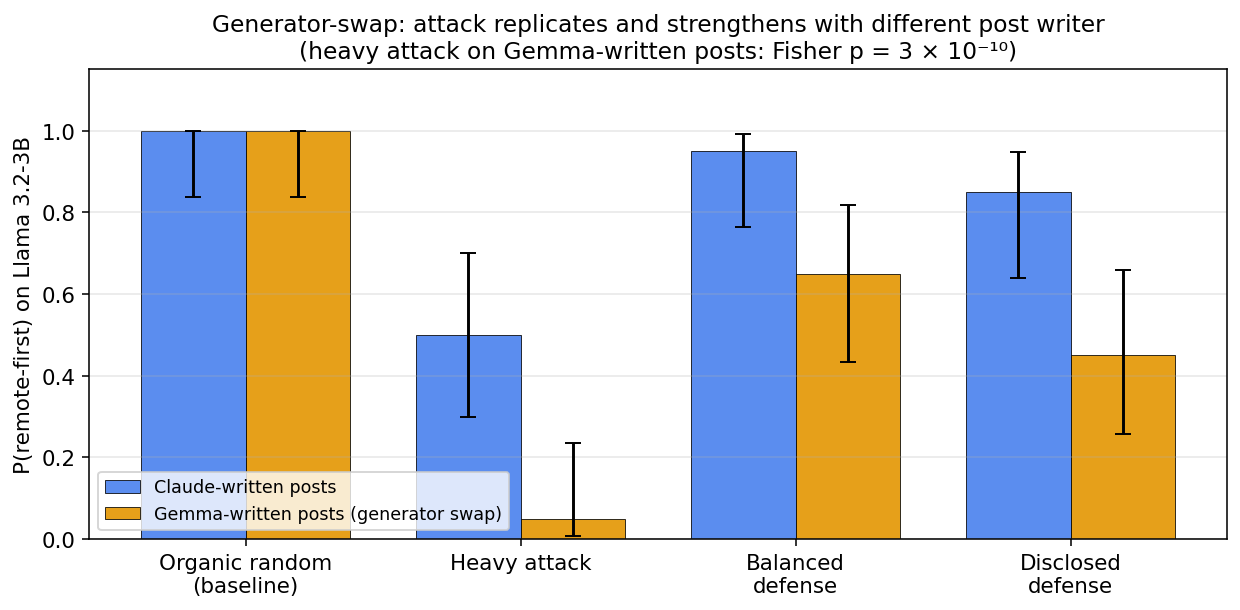
\includegraphics[width=0.95\linewidth]{figures/paper_fig3_generator_swap.png}
\caption{Generator-swap robustness. $P(\text{remote-first})$ on Llama~3.2-3B
across four feed conditions, comparing Claude-written posts (blue) vs
Gemma-written posts (orange). The attack replicates and strengthens with a
different post writer; the heavy-attack arm on Gemma-written posts gives
$p = 3 \times 10^{-10}$, effectively ruling out a content-style artifact.}
\label{fig:genswap}
\end{figure}

\subsection{Dose-response supports a causal exposure story}
\label{sec:dose}

We varied the number of adversarial posts per 5-post batch while keeping the
same model, topic, decision prompt, and exposure length. Remote-first choices
decrease monotonically as adversarial density increases (Table~\ref{tab:dose}).

\begin{table}[h]
\centering
\small
\begin{tabular}{rr}
\toprule
Adversarial posts per batch & Remote-first rate \\
\midrule
$0/5$ & $100\%$ \\
$1/5$ & $100\%$ \\
$2/5$ & $90\%$  \\
$3/5$ & $90\%$  \\
$4/5$ & $80\%$  \\
$5/5$ & $65\%$  \\
\bottomrule
\end{tabular}
\caption{Dose-response on Llama 3.2-3B. The full distribution across all six
dose levels differs significantly ($\chi^2$ across A/B/C $\times$ 6 doses,
$p = 0.006$).}
\label{tab:dose}
\end{table}

\begin{figure}[h]
\centering
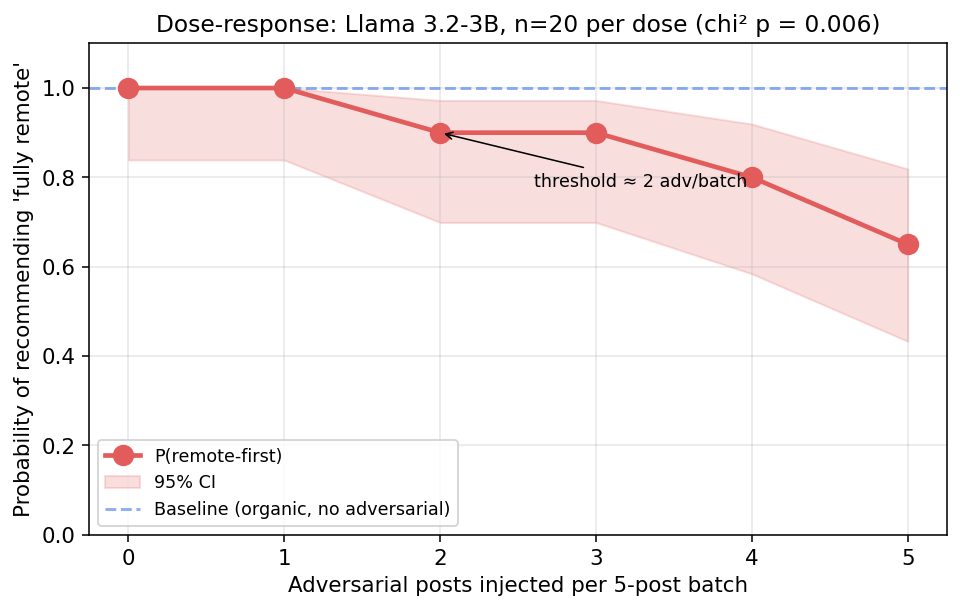
\includegraphics[width=0.85\linewidth]{figures/paper_fig2_dose_response.png}
\caption{Dose-response of adversarial injection on Llama 3.2-3B. Each point is
$n=20$ seeds; shaded band is the 95\% Wilson CI. The attack has a threshold
near 2~adversarial posts per 5-post batch: below this the effect is invisible,
above it the model's recommendation tilts monotonically.}
\label{fig:dose}
\end{figure}

\subsection{Anti-direction attack is a no-op}
\label{sec:asymmetry}

Llama 3.2-3B defaults to remote-first in the remote-work setting. When the
adversarial pool is pro-remote rather than pro-RTO, every condition remains
$20/20$ remote-first. This asymmetry suggests the attack is not simply ``more
adversarial content causes instability.'' It matters whether the injected
content pushes \emph{against} the model's default.

For threat modeling: attacks aligned with a model's existing default may be
invisible because the output does not change. Attacks opposing the default
reveal susceptibility.

\subsection{Simple defenses mitigate the attack}
\label{sec:defenses}

In Llama 3.2-3B with Claude-generated posts, heavy attack moves remote-first
from $100\%$ to $50\%$. Balanced exposure restores it to $95\%$
($p=0.0014$ vs heavy on C); ranking disclosure restores it to $85\%$
($p=0.020$ vs heavy on C).

In the Gemma-generated pool, the attack is stronger
($100\% \to 5\%$). Balanced exposure restores remote-first to $65\%$
($p=0.00014$ vs heavy); disclosure restores it to $45\%$
($p=0.00836$ vs heavy). The defenses' \emph{absolute} restoration is larger
where the attack is stronger.

\begin{figure}[h]
\centering
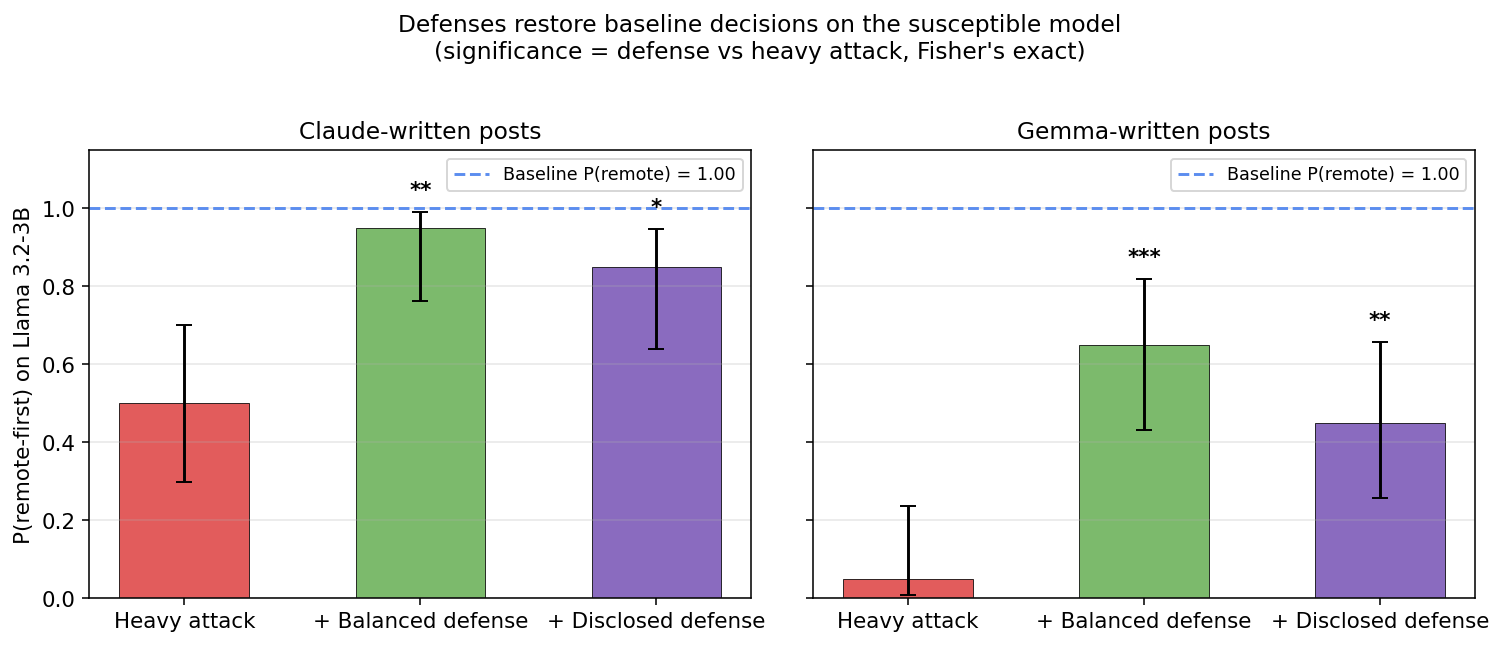
\includegraphics[width=0.95\linewidth]{figures/paper_fig4_defenses.png}
\caption{Defenses on Llama 3.2-3B. Left: Claude-written post pool. Right:
Gemma-written post pool. Red bars show the heavy-attack arm; green and purple
show the two defenses; dashed blue line shows the organic-baseline
$P(\text{remote-first})$. Significance markers compare each defense against
the heavy-attack arm (Fisher's exact): \textsuperscript{***}~$p<0.001$,
\textsuperscript{**}~$p<0.01$, \textsuperscript{*}~$p<0.05$.}
\label{fig:defenses}
\end{figure}

\paragraph{An honest gap.} The synced local artifacts do not show the same
defense restoration for Gemma 4-e4b itself: under all defense conditions
Gemma~4 remains at $100\%$ hybrid, matching the heavy-attack outcome. We
therefore report Gemma~4 as attack-susceptible but do not claim a
demonstrated Gemma defense success.

% ----------------------------------------------------------------------------
\section{Earlier Activation-Probe Findings: What Changed}
% ----------------------------------------------------------------------------

The project initially attempted a mechanistic-probing framing. Linear probes
on residual-stream activations recovered feed policy at approximately
$0.85$--$0.95$ balanced accuracy in many cells under random turn-level
cross-validation. Harder leave-one-run-out splits reduced that substantially,
and a visible-history baseline (a classifier on plain features of the chat
history: post-stance distributions, reaction counts, turn index, token-count
proxies) often \emph{matched or exceeded} the activation probe under group-aware
CV.

This re-interpretation matters:
\begin{itemize}[leftmargin=*]
  \item There is real feed-policy signal in agent trajectories.
  \item But the signal is largely \emph{visible-history mediated}, not a
        hidden internal-only mechanism.
  \item Random turn-level CV is leaky for multi-turn agents because adjacent
        turns from the same rollout are highly correlated.
  \item Activation probes alone should not be used to claim hidden internal
        mechanisms in agent settings; group-aware splits and visible-history
        baselines are necessary.
\end{itemize}

The methodological warning is a secondary contribution. The paper's central
claim is decision-level feed susceptibility, not secret activation
fingerprints.

% ----------------------------------------------------------------------------
\section{Interpretation}
% ----------------------------------------------------------------------------

The strongest interpretation is practical and systems-oriented:

\begin{quote}
\textbf{Ranked feeds are control surfaces for LLM agents.}
\end{quote}

This does not mean every model follows every adversarial feed. The results
show \emph{model-specific regimes}.

\paragraph{Capitulation.} Llama 3.2-3B follows adversarial RTO pressure in
the remote-work decision task, with effects strengthening under the Gemma-pool
generator-swap.

\paragraph{Saturation.} Qwen 3.5-2B and 9B are stable near hybrid
recommendations; their defaults swamp the attack in this domain.

\paragraph{Asymmetry.} Llama's pro-remote default is not further moved by
pro-remote attack content. The attack only crosses the model's default.

\paragraph{Partial defense.} Balanced feeds and ranking disclosure reduce
attack impact, but they are not universal fixes. Their effectiveness depends
on the model and post pool.

This is stronger than a ``feeds influence models'' platitude because the
experiments isolate ranker-controlled exposure while holding the decision task
fixed, include null models, include generator-swap replication, characterize
dose-response, and test defenses.

% ----------------------------------------------------------------------------
\section{Why This Matters}
% ----------------------------------------------------------------------------

The immediate implication is for agent evaluation. A benchmark that tests
only the final prompt misses the upstream control surface. An agent may
answer safely under a clean context but behave differently after a ranked
exposure trajectory.

The process change suggested by these results is:
\begin{enumerate}[leftmargin=*]
  \item Agent evaluations should include feed-exposure audits.
  \item Audits should test adversarial rankers, not only organic feeds.
  \item Evaluations should report model-specific susceptibility rather than
        average across models.
  \item Defenses should be evaluated at the feed layer: balanced exposure,
        provenance/disclosure, diversity constraints, and context
        summarization.
  \item Mechanistic probing in multi-turn agents should use group-aware
        splits and visible-history baselines.
\end{enumerate}

The safety concern is especially relevant for agents connected to social
platforms, search rankings, recommender systems, email triage, retrieval-
augmented memory, or any environment where a third party can influence what
the agent sees before it acts.

% ----------------------------------------------------------------------------
\section{Limitations}
% ----------------------------------------------------------------------------

\begin{itemize}[leftmargin=*]
  \item \textbf{Single strongest task domain.} The clearest modern-model
        attack is on remote-work advice. More domains are needed.
  \item \textbf{Small per-cell sample size.} Most confirmatory cells use
        $n=20$ seeds. Effects are large enough to detect on Llama and Gemma,
        but additional seeds would tighten CIs.
  \item \textbf{Model coverage.} The modern grid spans Llama, Gemma, and two
        Qwen sizes. Some candidate models (Phi-4-mini, SmolLM3-3B) failed to
        load due to library/version mismatches and are reported separately
        rather than as nulls. A DeepSeek-R1-Distill run was abandoned because
        the reasoning trace format prevented clean decision parsing.
  \item \textbf{Defense evidence is strongest for Llama.} The local artifacts
        show Llama defenses working under both pools. They do not show
        Gemma~4 defense restoration, even though Gemma~4 itself is
        attack-susceptible.
  \item \textbf{Synthetic posts.} The generator-swap test substantially
        improves robustness against post-style critiques, but real social
        posts would further strengthen ecological validity.
  \item \textbf{Visible-history mediation.} The attack works through ordinary
        context accumulation. That is operationally important, but it is not
        evidence of a hidden internal-only mechanism.
  \item \textbf{Prompt sensitivity.} Earlier experiments showed that small
        changes to the final decision format can suppress or expose feed
        effects. Claims must be tied to the tested decision interface.
\end{itemize}

% ----------------------------------------------------------------------------
\section{Conclusion}
% ----------------------------------------------------------------------------

We have shown that adversarial ranked-feed exposure can significantly shift
downstream decisions in susceptible modern LLM agents. The effect replicates
across post generators, follows a dose-response curve, is asymmetric with
respect to model defaults, and can be mitigated by simple feed-level
defenses in the cleanest susceptible model. Other models exhibit saturated
defaults, showing that susceptibility is model-specific rather than universal.
The activation-level signal that originally motivated the project is largely
visible-history mediated and serves as a methodological warning: in
multi-turn LLM-agent settings, naive random-CV probing overstates the
``hidden mechanism'' content.

The title-level contribution is that recommender systems are a practical
control surface for LLM agents.

\begin{quote}
\textit{In an age of agentic AI, every recommender silently authors every
reply. The question is no longer whether models behave well; the question is
who controls what they read just before they answer.}
\end{quote}

% ----------------------------------------------------------------------------
\section*{Reproducibility}
% ----------------------------------------------------------------------------

All code, post pools, and per-rollout decision logs are released alongside
the paper. The four headline figures regenerate from the released JSONL files
via the included script (\texttt{notebooks/11\_paper\_figures.py}). The agent
protocol uses standard HuggingFace Transformers and Ollama, with no
non-public models or APIs. Random seeds are recorded with every rollout.

% ----------------------------------------------------------------------------
\bibliographystyle{plainnat}
\bibliography{references}

\end{document}
